\section{Introduction}
\label{sec:introduction}

\subsection{Background}
Prostrate cancer is the second most common cancer
among men. Several screening methodologies exist for diagnosis of prostate cancer, however it is most commonly diagnosed by histopathology interpretation of Hematoxylin and Eosin (H \& E) stained tissue sections by pathologists under a microscope. Diagnosis of prostate cancer is carried out by examining the glandular architecture of the tissue sections. The diagnosis is done in the form of the Gleason grading system \cite{gleason1966classification} under which pathologists identify the malignancy of cancer areas in tissue images on a scale of 1 to 5. Gland distributions inside the tissue vary with the disease grade, and the morphological features of the glands vary with the stage of cancer. However, this is prone to subjectivity and has limited intra- and inter-pathologist reproducibility due to its heavy reliance on human interpretation. Even if only a single grade is desired, recent work has discovered that there is only a 60-70 \% agreement between pathologists on this grade.


Existing techniques to perform automated analysis of H \& E stained tissue have not had much accuracy expect in stylized toy cases. And because of the inter-disciplinary nature of the task, the problem has not attracted much attention. Most of the research has focused on distinguishing between Gleason grades (often between only two Gleason grades).In our work we focus on distinguishing cancerous tissue from non-cancerous tissue rather than distinguishing between Gleason grades for the tissue.

\subsection{Prostate Tissue Structure}
Normal Prostate tissue (shown in Figure \ref{fig:tissue_structure1}) is composed of gland units contained inside a fibromuscular region called stroma which holds the gland units together. Each gland unit is composed of rows of epithelial cells located around a duct, named the lumen. 

\begin{figure}[!htb]
\centering
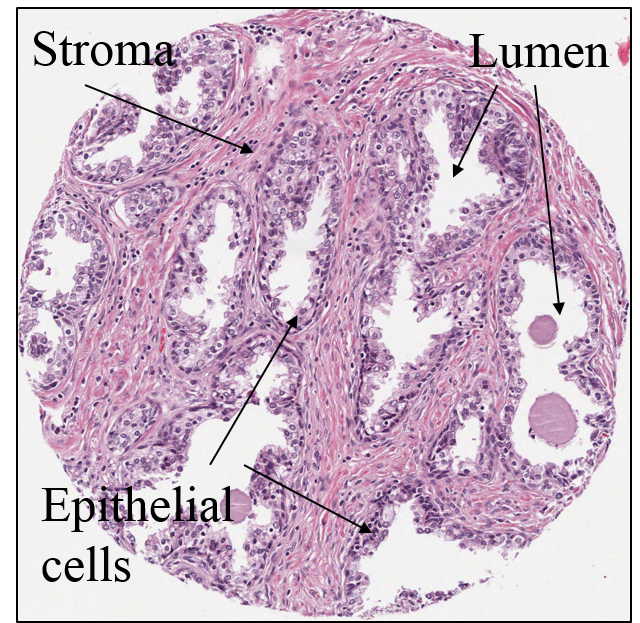
\includegraphics[scale=0.3]{figs/tissue_structure1.png}
\caption{Prostate Tissue Structure}\label{fig:tissue_structure1}
\centering
\end{figure}


Figure \ref{fig:tissue_types} shows non-cancerous and cancerous Prostate tissue. When cancer occurs the following changes take place in the tissue depending upon the level of malignancy:
\begin{enumerate}
\item[1.] Epithelial cells replicate in an uncontrolled way, disrupting the regular arrangement of gland units.
\item[2.] The glands in the cancerous region become small, regular, and more tightly packed as
cancer progresses from benign to highly malignant. While benign, healthy tissue has large and irregular lumen regions, higher grade cancers have small, narrow lumen regions.
\end{enumerate}




\begin{figure}[!htb]
\centering
\begin{minipage}[b]{.48\linewidth}
  \centering
  \centerline{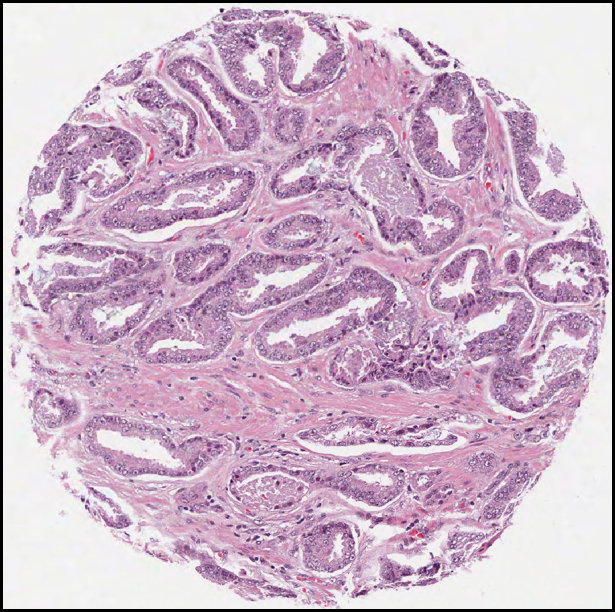
\includegraphics[scale=0.3]{figs/tissue_structure2.png}}
%  \vspace{1.5cm}
  \centerline{{Benign Tissue}\label{fig:tissue_structure2}}\medskip
\end{minipage}
\hfill
\begin{minipage}[b]{0.48\linewidth}
  \centering
  \centerline{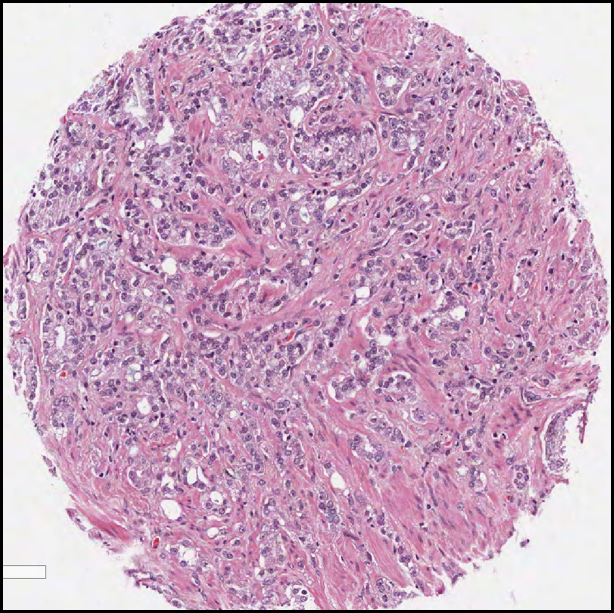
\includegraphics[scale=0.3]{figs/tissue_structure3.png}}
%  \vspace{1.5cm}
  \centerline{{Malignant Tissue}\label{fig:tissue_structure2}}\medskip
\end{minipage}
\caption{Structural changes in Prostate tissue when cancer occurs}
\label{fig:tissue_types}
\end{figure}

%\begin{figure}[!htb]
%\centering
%\captionsetup{justification=centering}
%\begin{subfigure}{.5\textwidth}
%	\centering
%	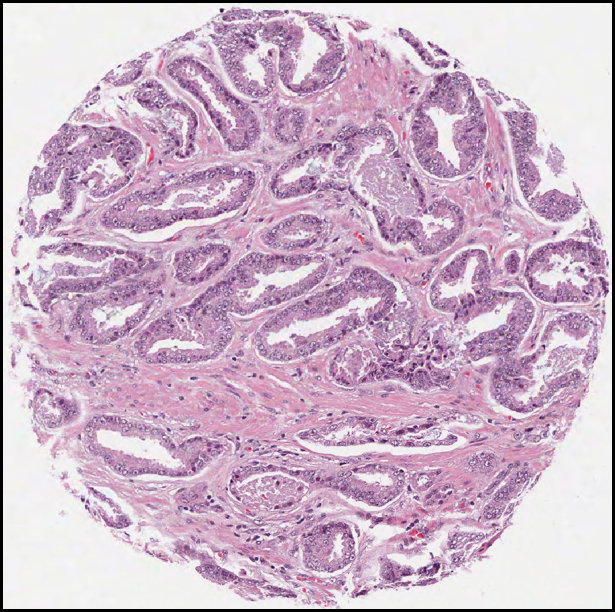
\includegraphics[scale=0.3]{figs/tissue_structure2.png}
%	\caption{Benign Tissue}\label{fig:tissue_structure2}
%	\centering
%\end{subfigure}
%\hfill
%\begin{subfigure}{.5\textwidth}
%	\centering
%	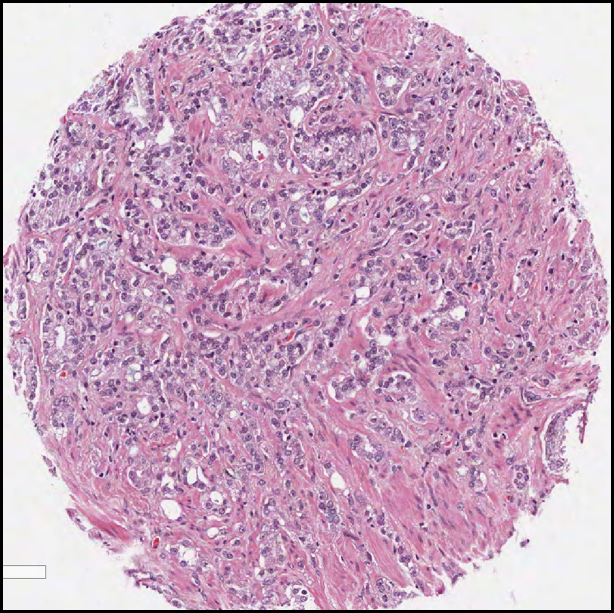
\includegraphics[scale=0.3]{figs/tissue_structure3.png}
%	\caption{Malignant Tissue}\label{fig:tissue_structure2}
%	\centering
%\end{subfigure}
%\caption{Structural changes in Prostate tissue when cancer occurs}
%\label{fig:tissue_types}
%\centering
%\end{figure}

These changes, along with different color values identifying different regions of interest ( lumen regions are white, stroma is pink and epithelial cells are usually a dark shade of purple ) can be used to build a classification system for separating non-cancerous and cancerous images.
